%%%% CAPÍTULO 2 - REVISÃO DA LITERATURA (OU REVISÃO BIBLIOGRÁFICA, ESTADO DA ARTE, ESTADO DO CONHECIMENTO)
%%
%% O autor deve registrar seu conhecimento sobre a literatura básica do assunto, discutindo e comentando a informação já publicada.
%% A revisão deve ser apresentada, preferencialmente, em ordem cronológica e por blocos de assunto, procurando mostrar a evolução do tema.
%% Título e rótulo de capítulo (rótulos não devem conter caracteres especiais, acentuados ou cedilha)
\chapter{Referencial te\'orico}\label{cap:referencialTeorico}

Esta seção descreve os principais tópicos teóricos envolvidos neste trabalho.

\section{Sistemas}

Um sistema, de acordo com o dicionário "Conjunto de elementos distintos, com características e funções específicas, organizadas de forma natural ou por meios artificiais"\cite{dicionário} é muito utilizado para nomear uma ampla gama de eventos naturais e artefatos artificiais criados a partir das interações de múltiplos componentes individuais com funções normalmente distintas com um efeito ou objetivo. Por exemplo, o sistema digestivo é composto por vários 

É comum atribuir a ideia de "sistema" a artefatos que são construídos pois esse termo é amplamente utilizado meio técnico para se referir a conceitos e cargos relacionados a área de computação. "Sistemas de informação", "analise de sistemas", "sistemas distribuídos" não são estranhos para profissionais da área e isso faz com que o termo acabe se tornando um sinônimo para software
\section{Hardware}

\section{Software}



\section{Sistemas Distribu\'idos}\label{sec:sistemasDistribuidos}

Sistemas Distribuídos são aplicações constituídas de elementos computacionais independentes, também conhecidos como nós, que cooperam entre si para fornecer um conjunto de funcionalidades que se apresentam para o usuário como um único sistema coerente\cite{van2017distributed}. Segundo essa definição, destacam-se duas características desses sistemas: a autonomia dos componentes(nós) que podem ser constituídos de processos de software ou dispositivos de hardware, e a necessidade de colaboração entre eles para criar a ilusão de um único sistema para quem o usa.

A necessidade de construir sistemas distribuídos emerge quando dois requisitos de projeto se mostram fundamentais: desempenho/escalabilidade e confiabilidade/disponibilidade. O primeiro requisito visa garantir que a aplicação vai ser capaz de atender uma grande quantidade de usuários ou aumente a complexidade computacional de suas funcionalidades sem que a mesma sofra com gargalos de desempenho. Quando distribuímos a carga computacional entre múltiplos nós, evita-se que um servidor seja sobrecarregado, evitando uma indisponibilidade completa do sistema devido a um ponto único de falha. O segundo objetivo é aprimorar a tolerância a falhas do sistema, onde a falha de um único nó (falha parcial) necessariamente compromete a disponibilidade total do serviço. Esse objetivo é atingido ao aplicarmos técnicas que gerarem redundância no sistema, dando capacidade ao mesmo de mascarar falhas e recuperar automaticamente a execução da operação do usuário final sem que ele perceba a interrupção. Esse princípio é conhecido como transparência de falhas.

\subsection{Middleware}\label{subsec:middleware}

É uma camada de software intermediária responsável pela comunicação entre os nós, sendo sua responsabilidade garantir a coerência e orquestrar as funções complexas do sistema sem externalizar a complexidade do funcionamento do mesmo para o usuário, sendo uma camada de software rodando sobre o sistema operacional de cada nó que fornece uma interface de uniforme de comunicação interprocesso, escalabilidade, segurança e disponibilidade\cite{astley2001middleware, van2017distributed}. 

O \textit{middleware} atua de forma análoga a um sistema operacional para um computador: ele gerencia os recursos do sistema distribuído e oferece às aplicações uma maneira de compartilhá-los e utilizá-los eficientemente através da rede. Seu principal objetivo é mascarar, da melhor forma possível, as diferenças de hardware e de sistemas operacionais, oferecendo uma interface de programação uniforme para as aplicações, conforme ilustrado na Figura \ref{fig:middleware}.

\begin{figure}[htb]%% Ambiente figure
    %\captionsetup{width=0.55\textwidth}%% Largura da legenda
    \caption{Um sistema distribuído organizado sobre uma camada de middleware que se extende para várias máquinas e oferece a mesma interface pra cada aplicação}%% Legenda
    \label{fig:middleware}%% Rótulo
    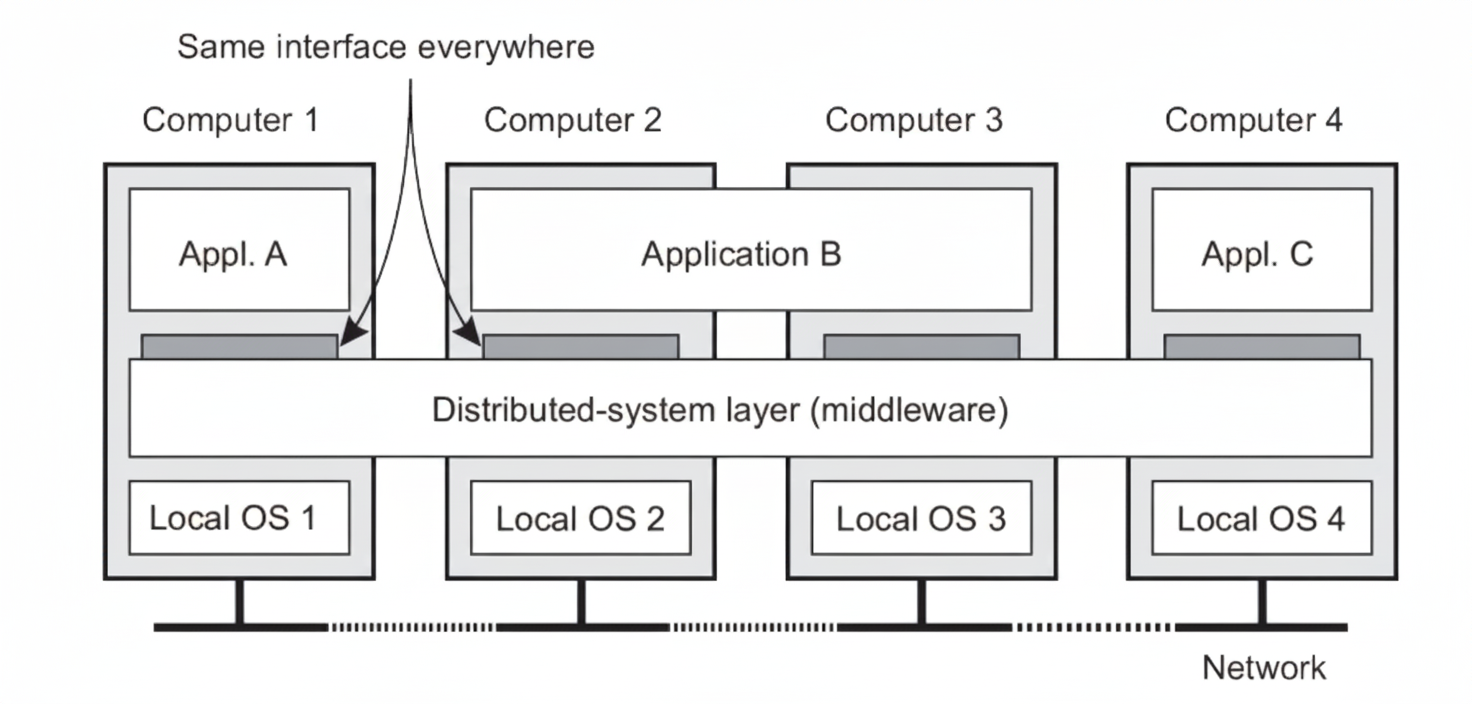
\includegraphics[scale=0.3]{figuras/conceitos/middleware.png}%% Dimensões e localização
    \fonte{Adaptado de \citeonline{van2017distributed}}%% Fonte
\end{figure}

Além do gerenciamento de recursos, o \textit{middleware} oferece um conjunto de serviços gerais para evitar que cada aplicação precise reimplementá-los. Esses serviços incluem:

\begin{itemize}
    \item Facilidades para comunicação entre aplicações;
    \item Serviços de segurança e confiabilidade;
    \item Mecanismos para mascarar e se recuperar de falhas;
    \item Suporte para a execução de transações atômicas distribuídas.
\end{itemize}

\subsection{Interoperabilidade}\label{subsec:interoperabilidade}

\subsection{Criptografia Assimétrica}\label{subsec:criptografiaAssimetrica}
    
\subsection{Engenharia Biomédica}\label{subsec:engBioMed}
\subsection{Biossinais}\label{subsec:ontologias}

"Sinais elétricos, mecânicos e químicos originados por seres vivos podem sempre ser de interesse para diagnósticos, monitoramento de pacientes e pesquisa biomédica"\cite{hadjileontiadis2006biosignals}. Esses Biossinais "carregam informação que é útil para a compreensão de mecanismos patológicos complexos subjacente ao comportamento dos sistemas vivos"\cite{liang2012biosignal}.

\subsection{Eletromiografia}\label{subsec:biossinais}

 O sinal de eletromiografia é composto pela variação potencial de grupos de fibras musculares organizadas em unidades funcionais chamada \textit{unidades motoras}\cite{de2006decomposition}. Esse sinal pode ser detectado através de métodos invasivos com eletrodos posicionados diretamente no tecido muscular, ou através de métodos não-invasivos com sensores posicionados na superfície da pele. 

 \begin{citacao}
Os ramos de uma fibra nervosa ativam a placa motora final de uma fibra muscular. Isso induz duas ondas de despolarização que viajam a uma velocidade de 3-6 m/s para cada extremidade da fibra muscular. O tecido entre e ao redor da fibra ativa é eletricamente condutor.

Sinais elétricos relacionados à despolarização da fibra podem, portanto, ser registrados por eletrodos a alguma distância da fibra: o EMG. A onda de despolarização também é conduzida para o interior da fibra por túbulos transversais muito finos, onde libera íons de cálcio que iniciam o processo de contração mecânica.

Este último processo é muito mais lento que a despolarização elétrica, que dura apenas 2 ms. Após uma única despolarização, a força máxima não é atingida antes de 20-150 ms, e o declínio gradual da força, devido à reabsorção dos íons de cálcio liberados, leva pelo menos o dobro desse tempo. \cite[p. 120-121]{hof1984emg}.
\end{citacao}

\subsection{Eletromiografia de Superfície(sEMG)}

\section{Normas, Padronizações e Leis}\label{sec:normas}

    \subsection{NBRISO 18308:2013}\label{subsec:NBRISO18308}
    
    \subsection{NBRISO/HL7 10781:2017}\label{subsec:NBRISO10781}



